\documentclass[12pt,a4paper]{article}
\usepackage[a4paper, margin=0.8in, headheight=14pt]{geometry}
\usepackage{fontspec}
\usepackage{unicode-math}
\setmainfont{TeX Gyre Pagella}
\setmonofont[Scale=0.88]{TeX Gyre Cursor}
\setmathfont{Latin Modern Math}

\usepackage{xcolor}
\usepackage{colortbl}
\usepackage{titlesec}
\usepackage{enumitem}
\usepackage{tabularx}
\usepackage{booktabs}
\usepackage{array}
\usepackage{amsmath}
\allowdisplaybreaks
\usepackage{tikz}
\usetikzlibrary{shapes.geometric, arrows.meta, positioning, calc, fit, decorations.pathreplacing, patterns}
\usepackage{tcolorbox}
\tcbuselibrary{skins, breakable}
\usepackage{hyperref}
\usepackage{fancyhdr}
\usepackage{graphicx}
\usepackage{microtype}
\hyphenpenalty=10000
\exhyphenpenalty=10000
\sloppy
\usepackage{caption}
\usepackage{setspace}
\usepackage{multirow}
\usepackage{tocloft}

% ─── Q&A helper ────────────────────────────────────────────────────────────────
\newcommand{\Q}[1]{\textbf{#1}\par\noindent\ignorespaces}

% ─── Colour Palette ────────────────────────────────────────────────────────────
\definecolor{myred}{RGB}{196,30,58}
\definecolor{mydark}{RGB}{30,30,50}
\definecolor{mygreen}{RGB}{14,120,80}
\definecolor{myteal}{RGB}{0,130,140}
\definecolor{myamber}{RGB}{220,130,20}
\definecolor{mypurple}{RGB}{90,40,140}
\definecolor{mygray}{RGB}{248,249,251}
\definecolor{mgframe}{RGB}{215,220,230}
\definecolor{watermark}{RGB}{145,150,170}
\definecolor{hdrred}{RGB}{250,232,235}
\definecolor{hdrgreen}{RGB}{220,244,233}
\definecolor{hdrteal}{RGB}{220,242,244}
\definecolor{hdramber}{RGB}{253,242,215}
\definecolor{hdrpurple}{RGB}{238,228,255}
\definecolor{hdrgray}{RGB}{238,240,245}
\definecolor{rowalt}{RGB}{250,251,253}

% ─── Section Formatting ────────────────────────────────────────────────────────
\titleformat{\section}
  {\large\bfseries\color{myred}}{\thesection.}{0.5em}{}
  [\vspace{1pt}{\color{myred}\rule{\linewidth}{0.8pt}}]
\titleformat{\subsection}
  {\normalsize\bfseries\color{myteal}}{\thesubsection}{0.5em}{}
\titlespacing*{\section}{0pt}{18pt}{7pt}
\titlespacing*{\subsection}{0pt}{11pt}{4pt}

% ─── Paragraph ─────────────────────────────────────────────────────────────────
\setlength{\parindent}{0pt}
\setlength{\parskip}{4pt}

% ─── TOC Styling ───────────────────────────────────────────────────────────────
\renewcommand{\cfttoctitlefont}{\large\bfseries\color{myred}}
\renewcommand{\cftaftertoctitle}{\par\noindent{\color{myred}\rule{\linewidth}{0.8pt}}}
\setlength{\cftbeforetoctitleskip}{0pt}
\setlength{\cftaftertoctitleskip}{6pt}
\renewcommand{\cftsecfont}{\normalsize\bfseries\color{mydark}}
\renewcommand{\cftsecpagefont}{\normalsize\bfseries\color{mydark}}
\renewcommand{\cftsecleader}{\cftdotfill{\cftdotsep}}
\setlength{\cftbeforesecskip}{7pt}
\renewcommand{\cftsubsecfont}{\small\color{mydark}}
\renewcommand{\cftsubsecpagefont}{\small\color{mydark}}
\setlength{\cftbeforesubsecskip}{3pt}
\setlength{\cftsubsecindent}{1.4em}

% ─── Table helpers ─────────────────────────────────────────────────────────────
\renewcommand{\arraystretch}{1.45}
\setlength{\tabcolsep}{6pt}
\arrayrulecolor{mydark}
\newcolumntype{B}[1]{>{\small\bfseries\raggedright\arraybackslash}m{#1}}
\newcolumntype{Y}{>{\small\raggedright\arraybackslash}X}
\renewcommand{\tabularxcolumn}[1]{m{#1}}

% ─── Header / Footer ───────────────────────────────────────────────────────────
\pagestyle{fancy}
\fancyhf{}
\fancyhead[L]{\small\color{myred}\textbf{EC303}\;\color{mydark}--- Signals and System}
\fancyhead[R]{\small\color{myteal}\textbf{Module 3 Notes}}
\fancyfoot[C]{\small\color{mydark}\thepage}
\fancyfoot[R]{\small\color{watermark}\textit{\copyright\ Biraj}}
\renewcommand{\headrulewidth}{0.5pt}
\renewcommand{\footrulewidth}{0.3pt}

% ─── Hyperref ──────────────────────────────────────────────────────────────────
\hypersetup{
  colorlinks=true, linkcolor=myteal, urlcolor=myteal,
  pdfauthor={Biraj Sarkar (CGEC)},
  pdftitle={EC303 --- Module 3 Notes: Fourier Analysis, Frequency Response and Signal Space}
}

% ─── tcolorbox styles ──────────────────────────────────────────────────────────
\tcbset{
  tikzbox/.style={
    colback=mygray, colframe=mgframe, boxrule=0.6pt, arc=4pt,
    left=8pt, right=8pt, top=6pt, bottom=6pt,
    colbacktitle=mgframe, coltitle=mydark,
    fonttitle=\small\bfseries
  },
  defbox/.style={
    colback=hdrgreen, colframe=mygreen, boxrule=0.8pt, arc=4pt,
    left=9pt, right=9pt, top=6pt, bottom=6pt,
    colbacktitle=mygreen, coltitle=white,
    fonttitle=\small\bfseries
  },
  formulabox/.style={
    colback=hdrteal, colframe=myteal, boxrule=0.8pt, arc=4pt,
    left=9pt, right=9pt, top=6pt, bottom=6pt,
    colbacktitle=myteal, coltitle=white,
    fonttitle=\small\bfseries
  },
  examplebox/.style={
    colback=hdramber, colframe=myamber, boxrule=0.8pt, arc=4pt,
    left=9pt, right=9pt, top=6pt, bottom=6pt,
    colbacktitle=myamber, coltitle=white,
    fonttitle=\small\bfseries
  },
  masonbox/.style={
    colback=hdrpurple, colframe=mypurple, boxrule=0.8pt, arc=4pt,
    left=9pt, right=9pt, top=6pt, bottom=6pt,
    colbacktitle=mypurple, coltitle=white,
    fonttitle=\small\bfseries
  },
  exambox/.style={
    colback=hdrpurple, colframe=mypurple, boxrule=1pt, arc=5pt,
    left=10pt, right=10pt, top=8pt, bottom=8pt,
    colbacktitle=mypurple, coltitle=white,
    fonttitle=\bfseries,
    breakable, title after break={\textbf{Frequently Asked / Viva Questions (contd.)}}
  }
}

\tcbset{breakable}
\tcbset{after={\color{black}}}

% ─── TikZ Global Styles ────────────────────────────────────────────────────────
\tikzset{
  sysblock/.style={draw=myteal, fill=hdrteal, thick, rectangle, rounded corners=3pt, minimum height=1cm, minimum width=2.4cm, align=center, font=\small\bfseries},
  circnode/.style={draw=myred, fill=hdrred, circle, thick, inner sep=1.5pt, font=\small\bfseries},
  arrowline/.style={-{Latex[length=2.5mm]}, thick, color=mydark},
  dashline/.style={thick, dashed, color=myteal}
}

% ─── Document ──────────────────────────────────────────────────────────────────
\begin{document}

% ─── Title Block ───────────────────────────────────────────────────────────────
\begin{center}
  {\Large\bfseries\color{myred} EC303 --- Signals and System}\\[4pt]
  {\large\bfseries\color{mydark} Module 3: Fourier Analysis, Frequency Response \& Signal Space}\\[3pt]
  {\small\color{watermark} Prepared by \textbf{Biraj Sarkar (CGEC)} $\cdot$ MAKAUT B.Tech ECE (2023--27)}\\[2pt]
  {\small\color{watermark} Authoritative Syllabus-Aligned Notes}
\end{center}
\vspace{-4pt}
\noindent{\color{myred}\rule{\linewidth}{1.2pt}}

% ─── Table of Contents ─────────────────────────────────────────────────────────
\tableofcontents
\vspace{10pt}
\noindent{\color{mgframe}\rule{\linewidth}{0.6pt}}

% ───────────────────────────────────────────────────────────────────────────────
\section{Eigenfunctions and Periodic Inputs to LSI Systems}
% ───────────────────────────────────────────────────────────────────────────────

\subsection{Eigenfunctions of Continuous-Time LSI Systems}

\begin{tcolorbox}[defbox, title={\textbf{Definition: Eigenfunction of an LSI System}}]
An input signal $x(t)$ is termed an \textbf{eigenfunction} of an LSI system $\mathcal{T}$ if the resulting output $y(t)$ is simply a scaled replica of the same input signal:
\begin{equation}
  y(t) = \mathcal{T}\{x(t)\} = \lambda \cdot x(t)
\end{equation}
where the complex scalar $\lambda \in \mathbb{C}$ is the corresponding \textbf{eigenvalue}.
\end{tcolorbox}

\textbf{Proof that Complex Exponentials are Eigenfunctions:}
Let the input to a continuous-time LSI system with impulse response $h(t)$ be the complex exponential $x(t) = e^{s t}$, where $s = \sigma + j\omega \in \mathbb{C}$. By the convolution integral:
\begin{align}
  y(t) &= \int_{-\infty}^{\infty} h(\tau) x(t - \tau) d\tau = \int_{-\infty}^{\infty} h(\tau) e^{s(t - \tau)} d\tau \\
  &= e^{st} \left[ \int_{-\infty}^{\infty} h(\tau) e^{-s\tau} d\tau \right]
\end{align}
Notice that the bracketed integral is purely a function of the complex frequency variable $s$, independent of time $t$. Defining the system transfer function $H(s) \triangleq \int_{-\infty}^\infty h(\tau) e^{-s\tau} d\tau$:
\begin{equation}
  y(t) = H(s) \cdot e^{st}
\end{equation}
For purely imaginary frequencies $s = j\omega$, the input is the harmonic phasor $x(t) = e^{j\omega t}$, yielding:
\begin{equation}
  y(t) = H(j\omega) \cdot e^{j\omega t}
\end{equation}
Thus, \textbf{complex exponentials are eigenfunctions of LSI systems}, and the corresponding eigenvalue is the system's \textbf{Frequency Response} $H(j\omega)$.

\subsection{Response to Periodic and Semi-Periodic Inputs}
By the principle of superposition, if a periodic input is decomposed into a sum of harmonically related complex exponentials:
\begin{equation}
  x(t) = \sum_{k=-\infty}^{\infty} c_k e^{j k \omega_0 t}
\end{equation}
The steady-state response of the LSI system is directly obtained by scaling each harmonic component by the frequency response evaluated at that specific harmonic:
\begin{equation}
  y(t) = \sum_{k=-\infty}^{\infty} c_k H(j k \omega_0) e^{j k \omega_0 t}
\end{equation}

\textbf{Semi-Periodic Inputs:}
A semi-periodic signal is one that is periodic for $t \ge 0$ but zero for $t < 0$, represented as $x(t) = p(t) u(t)$, where $p(t + T_0) = p(t)$. When applied to an LSI system:
\begin{itemize}[topsep=2pt, itemsep=2pt]
  \item The total response consists of a \textbf{transient response} $y_{tr}(t)$ and a \textbf{steady-state response} $y_{ss}(t)$:
  \begin{equation}
    y(t) = y_{tr}(t) + y_{ss}(t)
  \end{equation}
  \item For a BIBO stable system, the transient response decays exponentially to zero ($\lim_{t\to\infty} y_{tr}(t) = 0$), and the output asymptotically converges to the purely periodic steady-state response $y_{ss}(t)$.
\end{itemize}

% ───────────────────────────────────────────────────────────────────────────────
\section{The Frequency Response \texorpdfstring{$H(j\omega)$}{H(j omega)}}
% ───────────────────────────────────────────────────────────────────────────────

\subsection{Definition and Relation to Impulse Response}

\begin{tcolorbox}[defbox, title={\textbf{Definition: Frequency Response}}]
The \textbf{Frequency Response} $H(j\omega)$ of a continuous-time LSI system is the Continuous-Time Fourier Transform (CTFT) of its unit impulse response $h(t)$:
\begin{equation}
  H(j\omega) \triangleq \mathcal{F}\{h(t)\} = \int_{-\infty}^{\infty} h(t) e^{-j\omega t} dt
\end{equation}
Conversely, the impulse response is recovered via the Inverse Fourier Transform:
\begin{equation}
  h(t) = \frac{1}{2\pi} \int_{-\infty}^{\infty} H(j\omega) e^{j\omega t} d\omega
\end{equation}
\end{tcolorbox}

\subsection{Magnitude Response and Phase Response}
In polar form, $H(j\omega)$ is expressed as:
\begin{equation}
  H(j\omega) = |H(j\omega)| e^{j \angle H(j\omega)}
\end{equation}
where:
\begin{itemize}[topsep=2pt, itemsep=2pt]
  \item $|H(j\omega)|$ is the \textbf{Magnitude Response} (or amplitude gain) of the system at frequency $\omega$.
  \item $\angle H(j\omega) = \arg[H(j\omega)]$ is the \textbf{Phase Response} (phase shift) imparted to the input phasor.
  \item \textbf{Group Delay $\tau_g(\omega)$:} The time delay experienced by a narrow-band signal envelope centered at frequency $\omega$:
  \begin{equation}
    \tau_g(\omega) \triangleq -\frac{d}{d\omega} \angle H(j\omega)
  \end{equation}
\end{itemize}

\textbf{Symmetry Properties for Real Impulse Response $h(t) \in \mathbb{R}$:}
\begin{enumerate}[topsep=2pt, itemsep=2pt]
  \item Conjugate symmetry: $H(-j\omega) = H^*(j\omega)$.
  \item Even magnitude symmetry: $|H(-j\omega)| = |H(j\omega)|$.
  \item Odd phase symmetry: $\angle H(-j\omega) = -\angle H(j\omega)$.
\end{enumerate}

\begin{tcolorbox}[examplebox, title={\textbf{Sinusoidal Steady-State Response}}]
If the input to an LSI system is a real sinusoid $x(t) = A \cos(\omega_0 t + \theta)$, the steady-state output is:
\begin{equation}
  y(t) = A |H(j\omega_0)| \cos\big(\omega_0 t + \theta + \angle H(j\omega_0)\big)
\end{equation}
The frequency remains completely unchanged; the system only scales the amplitude by $|H(j\omega_0)|$ and shifts the phase by $\angle H(j\omega_0)$.
\end{tcolorbox}

% ───────────────────────────────────────────────────────────────────────────────
\section{Continuous-Time Fourier Series (CTFS)}
% ───────────────────────────────────────────────────────────────────────────────

\subsection{Dirichlet Conditions for Convergence}
A periodic signal $x(t)$ with fundamental period $T_0$ and fundamental frequency $\omega_0 = 2\pi / T_0$ can be expanded in a Fourier series if it satisfies the \textbf{Dirichlet Conditions}:
\begin{enumerate}[topsep=2pt, itemsep=2pt]
  \item \textbf{Absolute Integrability:} Over any single period $T_0$, $\int_{T_0} |x(t)| dt < \infty$.
  \item \textbf{Bounded Variation:} $x(t)$ has a finite number of local maxima and minima within any single period.
  \item \textbf{Finite Discontinuities:} $x(t)$ has a finite number of discontinuities within any period, and each discontinuity is finite (bounded jump).
\end{enumerate}
At a point of finite discontinuity $t_0$, the Fourier series converges to the arithmetic mean of the left- and right-hand limits: $\frac{x(t_0^+) + x(t_0^-)}{2}$.

\subsection{Three Formulations of Fourier Series}

\par\vspace{6pt}\noindent
\begingroup
\setlength{\tabcolsep}{5pt}
\setlength{\extrarowheight}{3pt}
\renewcommand{\arraystretch}{1.4}
\begin{tabularx}{\linewidth}{|B{4cm}|Y|Y|}
\hline
\textbf{Representation} & \textbf{Synthesis Equation} & \textbf{Analysis / Coefficient Equations} \\
\hline
Trigonometric Fourier Series (TFS) & $x(t) = a_0 + \sum_{n=1}^\infty [a_n \cos(n\omega_0 t) + b_n \sin(n\omega_0 t)]$ & $a_0 = \frac{1}{T_0} \int_{T_0} x(t) dt$, \par $a_n = \frac{2}{T_0} \int_{T_0} x(t) \cos(n\omega_0 t) dt$, \par $b_n = \frac{2}{T_0} \int_{T_0} x(t) \sin(n\omega_0 t) dt$ \\
\hline
Compact / Polar Form & $x(t) = C_0 + \sum_{n=1}^\infty C_n \cos(n\omega_0 t + \theta_n)$ & $C_0 = a_0$, \quad $C_n = \sqrt{a_n^2 + b_n^2}$, \par $\theta_n = -\tan^{-1}(b_n / a_n)$ \\
\hline
Exponential / Complex Form (EFS) & $x(t) = \sum_{k=-\infty}^\infty c_k e^{j k \omega_0 t}$ & $c_k = \frac{1}{T_0} \int_{T_0} x(t) e^{-j k \omega_0 t} dt$ \\
\hline
\end{tabularx}
\endgroup

\subsection{Inter-Relationship Between TFS and EFS Coefficients}
\begin{align}
  c_0 &= a_0 = C_0 \\
  c_k &= \frac{a_k - j b_k}{2} = \frac{C_k}{2} e^{j\theta_k}, \qquad c_{-k} = c_k^* = \frac{a_k + j b_k}{2} = \frac{C_k}{2} e^{-j\theta_k} \\
  a_k &= c_k + c_{-k} = 2 \text{Re}\{c_k\}, \qquad b_k = j(c_k - c_{-k}) = -2 \text{Im}\{c_k\}
\end{align}

\subsection{Gibbs Phenomenon}
When a discontinuous signal (such as a square wave) is approximated by a truncated Fourier series with $N$ harmonics, an oscillatory overshoot occurs in the immediate vicinity of the discontinuity. As $N \to \infty$, the overshoot does not disappear; its width narrows to zero, but its peak amplitude approaches a fixed constant:
\begin{equation}
  \text{Overshoot Percentage} = \frac{\frac{2}{\pi} \int_0^\pi \frac{\sin x}{x} dx - 1}{1} \approx 8.95\% \approx 9\% \text{ of the jump discontinuity}
\end{equation}

% ───────────────────────────────────────────────────────────────────────────────
\section{Continuous-Time Fourier Transform (CTFT)}
% ───────────────────────────────────────────────────────────────────────────────

\subsection{Transition from Fourier Series to Fourier Transform}
An aperiodic signal $x(t)$ can be viewed as the limiting case of a periodic signal as the period $T_0 \to \infty$. In this limit:
\begin{itemize}[topsep=2pt, itemsep=2pt]
  \item The fundamental frequency $\omega_0 = 2\pi / T_0 \to d\omega$ becomes an infinitesimal differential.
  \item The discrete harmonic frequencies $k \omega_0 \to \omega$ merge into a continuous frequency continuum.
  \item The discrete spectrum $T_0 c_k$ transforms into the continuous spectral density $X(j\omega)$.
\end{itemize}

\begin{tcolorbox}[formulabox, title={\textbf{The Continuous-Time Fourier Transform (CTFT) Pair}}]
\begin{align}
  \textbf{Analysis (Forward CTFT):} \quad &X(j\omega) = \mathcal{F}\{x(t)\} = \int_{-\infty}^{\infty} x(t) e^{-j\omega t} dt \\
  \textbf{Synthesis (Inverse CTFT):} \quad &x(t) = \mathcal{F}^{-1}\{X(j\omega)\} = \frac{1}{2\pi} \int_{-\infty}^{\infty} X(j\omega) e^{j\omega t} d\omega
\end{align}
\end{tcolorbox}

\subsection{Properties of CTFT}

\par\vspace{6pt}\noindent
\begingroup
\setlength{\tabcolsep}{5pt}
\setlength{\extrarowheight}{3pt}
\renewcommand{\arraystretch}{1.4}
\begin{tabularx}{\linewidth}{|B{3.8cm}|B{4.5cm}|Y|}
\hline
\textbf{Property} & \textbf{Time Domain $x(t)$} & \textbf{Frequency Domain $X(j\omega)$} \\
\hline
Linearity & $a x_1(t) + b x_2(t)$ & $a X_1(j\omega) + b X_2(j\omega)$ \\
\hline
Time Shifting & $x(t - t_0)$ & $X(j\omega) e^{-j\omega t_0}$ \\
\hline
Frequency Shifting (Modulation) & $x(t) e^{j\omega_0 t}$ & $X(j(\omega - \omega_0))$ \\
\hline
Time Scaling & $x(at) \quad (a \ne 0)$ & $\frac{1}{|a|} X\left(j\frac{\omega}{a}\right)$ \\
\hline
Time Reversal & $x(-t)$ & $X(-j\omega) = X^*(j\omega) \quad (\text{if } x(t)\in\mathbb{R})$ \\
\hline
Duality & $X(jt)$ & $2\pi x(-\omega)$ \\
\hline
Time Differentiation & $\frac{d^n x(t)}{dt^n}$ & $(j\omega)^n X(j\omega)$ \\
\hline
Time Integration & $\int_{-\infty}^t x(\tau) d\tau$ & $\frac{1}{j\omega} X(j\omega) + \pi X(0) \delta(\omega)$ \\
\hline
Time Convolution & $x_1(t) * x_2(t)$ & $X_1(j\omega) \cdot X_2(j\omega)$ \\
\hline
Frequency Convolution (Multiplication) & $x_1(t) \cdot x_2(t)$ & $\frac{1}{2\pi} \big[ X_1(j\omega) * X_2(j\omega) \big]$ \\
\hline
\end{tabularx}
\endgroup

\subsection{Fourier Domain Duality}
The mathematical symmetry between the analysis and synthesis integrals leads to the \textbf{Duality Property}:
\begin{equation}
  \text{If } \mathcal{F}\{x(t)\} = X(j\omega), \quad \text{then } \mathcal{F}\{X(jt)\} = 2\pi x(-\omega)
\end{equation}
\textbf{Example:} Since a rectangular pulse in time transforms into a sinc function in frequency:
\begin{equation}
  \text{rect}\left(\frac{t}{\tau}\right) \iff \tau \text{sinc}\left(\frac{\omega\tau}{2\pi}\right)
\end{equation}
By duality, a sinc pulse in time transforms into an ideal rectangular spectrum in frequency:
\begin{equation}
  W \text{sinc}\left(\frac{Wt}{2\pi}\right) \iff 2\pi \cdot \text{rect}\left(\frac{\omega}{W}\right)
\end{equation}
This establishes that ideal bandlimited filtering in frequency corresponds to infinite sinc impulse responses in time.

% ───────────────────────────────────────────────────────────────────────────────
\section{Parseval's Theorem and Energy Spectral Density}
% ───────────────────────────────────────────────────────────────────────────────

\begin{tcolorbox}[formulabox, title={\textbf{Parseval's Energy Theorem}}]
\textbf{For Continuous-Time Fourier Transform:}
Total signal energy $E$ calculated in the time domain equals the energy integrated across all frequencies:
\begin{equation}
  E = \int_{-\infty}^{\infty} |x(t)|^2 dt = \frac{1}{2\pi} \int_{-\infty}^{\infty} |X(j\omega)|^2 d\omega = \int_{-\infty}^{\infty} |X(f)|^2 df
\end{equation}
where $f = \omega / 2\pi$ is frequency in Hertz.

\textbf{For Periodic Signals (CTFS):}
The average power $P$ equals the sum of the average powers in all individual harmonic components:
\begin{equation}
  P = \frac{1}{T_0} \int_{T_0} |x(t)|^2 dt = \sum_{k=-\infty}^{\infty} |c_k|^2 = C_0^2 + \frac{1}{2}\sum_{n=1}^{\infty} C_n^2
\end{equation}
\end{tcolorbox}

\textbf{Energy Spectral Density (ESD):}
The quantity $S_{xx}(\omega) \triangleq |X(j\omega)|^2$ represents the distribution of energy per unit frequency (in Joules/(rad/s)). When a signal passes through an LSI system:
\begin{equation}
  Y(j\omega) = X(j\omega) H(j\omega) \implies S_{yy}(\omega) = |Y(j\omega)|^2 = |H(j\omega)|^2 S_{xx}(\omega)
\end{equation}

% ───────────────────────────────────────────────────────────────────────────────
\section{Discrete-Time Fourier Transform (DTFT) \& Discrete Fourier Transform (DFT)}
% ───────────────────────────────────────────────────────────────────────────────

\subsection{Discrete-Time Fourier Transform (DTFT)}
The DTFT applies to infinite-length discrete-time sequences $x[n]$.

\begin{tcolorbox}[defbox, title={\textbf{Definition: DTFT and Inverse DTFT}}]
\begin{align}
  \textbf{Forward DTFT (Analysis):} \quad &X(e^{j\Omega}) = \sum_{n=-\infty}^{\infty} x[n] e^{-j\Omega n} \\
  \textbf{Inverse DTFT (Synthesis):} \quad &x[n] = \frac{1}{2\pi} \int_{-\pi}^{\pi} X(e^{j\Omega}) e^{j\Omega n} d\Omega
\end{align}
\end{tcolorbox}

\textbf{Fundamental Property: $2\pi$-Periodicity in Frequency:}
Since $e^{-j(\Omega + 2\pi) n} = e^{-j\Omega n} e^{-j 2\pi n} = e^{-j\Omega n} \cdot 1$:
\begin{equation}
  X(e^{j(\Omega + 2\pi)}) = X(e^{j\Omega})
\end{equation}
All distinct frequency information is fully contained within any interval of length $2\pi$, conventionally chosen as $[-\pi, \pi]$ or $[0, 2\pi]$.

\subsection{Discrete Fourier Transform (DFT)}
The DFT operates on finite-duration discrete-time sequences of length $N$, producing an $N$-point discrete frequency spectrum suitable for digital computer computation.

\begin{tcolorbox}[defbox, title={\textbf{Definition: Discrete Fourier Transform (DFT) Pair}}]
Let $x[n]$ be an $N$-point sequence defined for $n = 0, 1, \dots, N-1$.
\begin{align}
  \textbf{DFT (Analysis):} \quad &X[k] = \sum_{n=0}^{N-1} x[n] W_N^{kn}, \qquad k = 0, 1, \dots, N-1 \\
  \textbf{IDFT (Synthesis):} \quad &x[n] = \frac{1}{N} \sum_{k=0}^{N-1} X[k] W_N^{-kn}, \qquad n = 0, 1, \dots, N-1
\end{align}
where the \textbf{Twiddle Factor} is $W_N \triangleq e^{-j\frac{2\pi}{N}}$.
\end{tcolorbox}

\subsection{Relation Between DTFT and DFT}
The DFT values $X[k]$ are exact samples of the continuous DTFT $X(e^{j\Omega})$ evaluated at $N$ uniformly spaced points along the unit circle:
\begin{equation}
  X[k] = \left. X(e^{j\Omega}) \right|_{\Omega = \frac{2\pi k}{N}}, \qquad k = 0, 1, \dots, N-1
\end{equation}

% ───────────────────────────────────────────────────────────────────────────────
\section{Signal Space and Orthogonal Bases}
% ───────────────────────────────────────────────────────────────────────────────

\subsection{The Signal Space Concept (Hilbert Space $L^2$)}
Signals can be viewed as vectors residing in an infinite-dimensional vector space known as a \textbf{Hilbert Space} $\mathcal{H} = L^2[a,b]$. The geometric concepts of length, distance, and angle in Euclidean space generalize directly to signals:

\begin{itemize}[topsep=2pt, itemsep=2pt]
  \item \textbf{Inner Product $\langle x, y \rangle$:} The inner product of two signals $x(t)$ and $y(t)$ over interval $[t_1, t_2]$ is:
  \begin{equation}
    \langle x, y \rangle \triangleq \int_{t_1}^{t_2} x(t) y^*(t) dt
  \end{equation}
  \item \textbf{Signal Norm (Magnitude/Length):} The norm $\|x\|$ is defined as:
  \begin{equation}
    \|x\| \triangleq \sqrt{\langle x, x \rangle} = \left[ \int_{t_1}^{t_2} |x(t)|^2 dt \right]^{1/2} = \sqrt{E_x}
  \end{equation}
  where $E_x$ is the total energy of the signal.
  \item \textbf{Metric (Distance between Signals):} $d(x, y) = \|x - y\| = \sqrt{\int_{t_1}^{t_2} |x(t) - y(t)|^2 dt}$.
\end{itemize}

\subsection{Orthogonality and Orthonormal Bases}

\begin{tcolorbox}[defbox, title={\textbf{Definition: Orthogonal and Orthonormal Signal Sets}}]
A set of basis functions $\{\phi_1(t), \phi_2(t), \dots, \phi_N(t)\}$ is:
\begin{enumerate}[topsep=2pt, itemsep=2pt]
  \item \textbf{Orthogonal} if the inner product of distinct basis functions is strictly zero:
  \begin{equation}
    \langle \phi_i, \phi_j \rangle = \int_{t_1}^{t_2} \phi_i(t) \phi_j^*(t) dt = \begin{cases} 0, & i \ne j \\ E_i \ne 0, & i = j \end{cases}
  \end{equation}
  \item \textbf{Orthonormal} if it is orthogonal and every basis function has unit energy ($E_i = 1$):
  \begin{equation}
    \langle \phi_i, \phi_j \rangle = \delta_{ij} = \begin{cases} 1, & i = j \\ 0, & i \ne j \end{cases}
  \end{equation}
  where $\delta_{ij}$ is the Kronecker delta.
\end{enumerate}
\end{tcolorbox}

\subsection{Generalized Fourier Series Expansion}
Any arbitrary signal $x(t) \in \mathcal{H}$ can be represented as a linear combination of orthonormal basis functions:
\begin{equation}
  x(t) = \sum_{k=1}^{\infty} c_k \phi_k(t)
\end{equation}
Taking the inner product of both sides with $\phi_m(t)$:
\begin{equation}
  \langle x, \phi_m \rangle = \left\langle \sum_{k=1}^{\infty} c_k \phi_k, \phi_m \right\rangle = \sum_{k=1}^{\infty} c_k \langle \phi_k, \phi_m \rangle = \sum_{k=1}^{\infty} c_k \delta_{km} = c_m
\end{equation}
Hence, the projection coefficients are given by the projection integral:
\begin{equation}
  c_k = \langle x, \phi_k \rangle = \int_{t_1}^{t_2} x(t) \phi_k^*(t) dt
\end{equation}

\textbf{Generalized Parseval's Identity:}
If the basis $\{\phi_k(t)\}$ is complete:
\begin{equation}
  \|x\|^2 = \int_{t_1}^{t_2} |x(t)|^2 dt = \sum_{k=1}^{\infty} |c_k|^2
\end{equation}
The continuous-time Exponential Fourier Series is simply a special case where the orthonormal basis is $\phi_k(t) = \frac{1}{\sqrt{T_0}} e^{j k \omega_0 t}$ over interval $[0, T_0]$.

\begin{tcolorbox}[tikzbox, title={\textbf{TikZ Illustration: Signal Projection onto Orthogonal Basis Axes}}]
\begin{center}
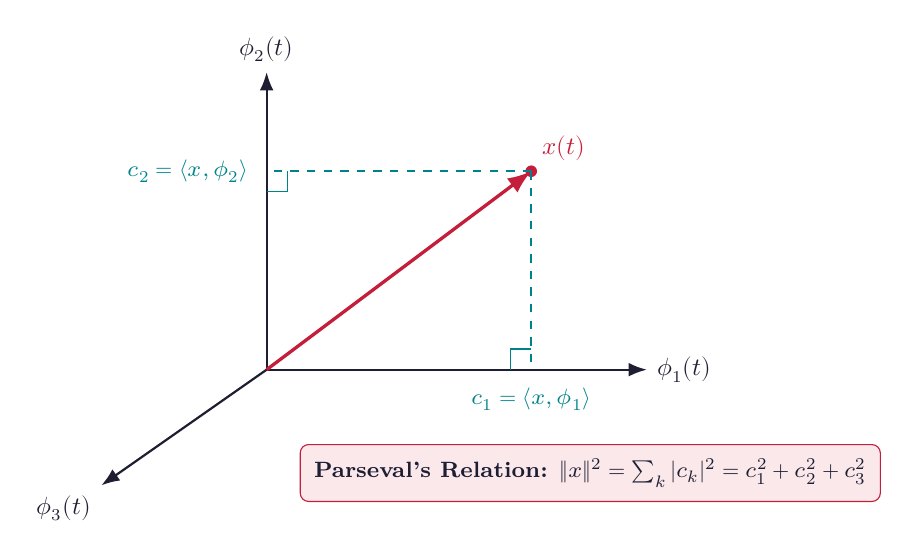
\begin{tikzpicture}[>=Latex, scale=1.05, font=\small]
  % Orthogonal Axes
  \draw[->, thick, color=mydark] (0,0) -- (4.6,0) node[right, font=\small\bfseries] {$\phi_1(t)$};
  \draw[->, thick, color=mydark] (0,0) -- (0,3.6) node[above, font=\small\bfseries] {$\phi_2(t)$};
  \draw[->, thick, color=mydark] (0,0) -- (-2.0,-1.4) node[below left, font=\small\bfseries] {$\phi_3(t)$};

  % Signal vector x(t)
  \draw[very thick, myred, -{Latex[length=3mm]}] (0,0) -- (3.2, 2.4) node[above right, font=\small\bfseries, color=myred] {$x(t)$};
  \fill[myred] (3.2, 2.4) circle (2pt);

  % Orthogonal Projections
  \draw[dashed, myteal, thick] (3.2, 2.4) -- (3.2, 0) node[below=3pt, color=myteal, font=\footnotesize\bfseries] {$c_1 = \langle x, \phi_1 \rangle$};
  \draw[dashed, myteal, thick] (3.2, 2.4) -- (0, 2.4) node[left=3pt, color=myteal, font=\footnotesize\bfseries] {$c_2 = \langle x, \phi_2 \rangle$};

  % Right angle indicator
  \draw[myteal] (3.2, 0.25) -- (2.95, 0.25) -- (2.95, 0);
  \draw[myteal] (0.25, 2.4) -- (0.25, 2.15) -- (0, 2.15);

  % Energy Formulation Box (Parseval's relation)
  \node[draw=myred, fill=hdrred, rounded corners=3pt, inner sep=5pt, font=\footnotesize\bfseries, text=mydark, anchor=west] at (0.4, -1.25) {
    Parseval's Relation: $\|x\|^2 = \sum_{k} |c_k|^2 = c_1^2 + c_2^2 + c_3^2$
  };
\end{tikzpicture}
\end{center}
\end{tcolorbox}

% ───────────────────────────────────────────────────────────────────────────────
% QUICK REVISION PAGE
% ───────────────────────────────────────────────────────────────────────────────
\newpage
\begin{center}
  {\Large\bfseries\color{myred} Quick Revision \& Examination Compendium}\\[3pt]
  {\small\color{watermark}\textbf{Module 3: Fourier Analysis, Frequency Response \& Signal Space}}
\end{center}
\vspace{-2pt}
\noindent{\color{myred}\rule{\linewidth}{0.8pt}}

\begin{tcolorbox}[formulabox, title={\textbf{Key Formulas at a Glance}}]
\par\vspace{4pt}\noindent
\begingroup
\setlength{\tabcolsep}{5pt}
\setlength{\extrarowheight}{3pt}
\renewcommand{\arraystretch}{1.4}
\begin{tabularx}{\linewidth}{|B{4.5cm}|Y|}
\hline
\textbf{Transform / Theorem} & \textbf{Definitive Mathematical Formula} \\
\hline
Frequency Response $H(j\omega)$ & $H(j\omega) = \int_{-\infty}^{\infty} h(t) e^{-j\omega t} dt = |H(j\omega)| e^{j\angle H(j\omega)}$ \\
\hline
Group Delay $\tau_g(\omega)$ & $\tau_g(\omega) = -\frac{d}{d\omega} \angle H(j\omega)$ \\
\hline
Exponential Fourier Series & $x(t) = \sum_{k=-\infty}^\infty c_k e^{j k \omega_0 t}, \quad c_k = \frac{1}{T_0} \int_{T_0} x(t) e^{-j k \omega_0 t} dt$ \\
\hline
CTFT Analysis / Synthesis & $X(j\omega) = \int_{-\infty}^\infty x(t) e^{-j\omega t} dt, \quad x(t) = \frac{1}{2\pi}\int_{-\infty}^\infty X(j\omega) e^{j\omega t} d\omega$ \\
\hline
CTFT Duality Property & $\mathcal{F}\{X(jt)\} = 2\pi x(-\omega)$ \\
\hline
CTFT Convolution & $\mathcal{F}\{x_1(t) * x_2(t)\} = X_1(j\omega) \cdot X_2(j\omega)$ \\
\hline
CTFT Multiplication & $\mathcal{F}\{x_1(t) \cdot x_2(t)\} = \frac{1}{2\pi} [X_1(j\omega) * X_2(j\omega)]$ \\
\hline
Parseval's Theorem (CTFT) & $\int_{-\infty}^\infty |x(t)|^2 dt = \frac{1}{2\pi} \int_{-\infty}^\infty |X(j\omega)|^2 d\omega$ \\
\hline
DTFT Analysis / Synthesis & $X(e^{j\Omega}) = \sum_n x[n] e^{-j\Omega n}, \quad x[n] = \frac{1}{2\pi}\int_{-\pi}^\pi X(e^{j\Omega}) e^{j\Omega n} d\Omega$ \\
\hline
DFT Analysis / Synthesis & $X[k] = \sum_{n=0}^{N-1} x[n] W_N^{kn}, \quad x[n] = \frac{1}{N} \sum_{k=0}^{N-1} X[k] W_N^{-kn}$ \\
\hline
Orthogonality Condition & $\langle \phi_i, \phi_j \rangle = \int \phi_i(t) \phi_j^*(t) dt = \delta_{ij} \|\phi_i\|^2$ \\
\hline
\end{tabularx}
\endgroup
\end{tcolorbox}

\begin{tcolorbox}[defbox, title={\textbf{One-Line Definitions for Rapid Review}}]
\par\vspace{4pt}\noindent
\begingroup
\setlength{\tabcolsep}{5pt}
\setlength{\extrarowheight}{3pt}
\renewcommand{\arraystretch}{1.35}
\begin{tabularx}{\linewidth}{|B{4.2cm}|Y|}
\hline
\textbf{Term} & \textbf{Definitive Technical Meaning} \\
\hline
Eigenfunction & A signal that when fed into an LSI system produces an output that is an exact scalar multiple of itself. \\
\hline
Frequency Response & The Fourier transform of the unit impulse response, expressing gain and phase shift vs frequency. \\
\hline
Group Delay & The negative derivative of phase with respect to angular frequency, indicating envelope propagation delay. \\
\hline
Dirichlet Conditions & Sufficient mathematical conditions (integrability, bounded extrema, finite jumps) for Fourier series convergence. \\
\hline
Gibbs Phenomenon & The persistent $\approx 9\%$ overshoot near step discontinuities in truncated Fourier series approximations. \\
\hline
Duality Property & The mathematical equivalence between time and frequency roles arising from symmetrical Fourier integrals. \\
\hline
Energy Spectral Density & The distribution of total signal energy as a function of continuous frequency, defined as $|X(j\omega)|^2$. \\
\hline
DTFT Periodicity & The inherent $2\pi$-periodicity of the discrete-time Fourier transform due to discrete sample spacing. \\
\hline
Twiddle Factor & The complex root of unity $W_N = e^{-j 2\pi / N}$ utilized in discrete Fourier transform calculations. \\
\hline
Hilbert Space & A complete vector space equipped with an inner product that defines length, distance, and angle for signals. \\
\hline
\end{tabularx}
\endgroup
\end{tcolorbox}

\begin{tcolorbox}[exambox, title={\textbf{Frequently Asked / Viva Questions}}]
\begin{enumerate}[topsep=0pt, label=\textbf{Q\arabic*.}, itemsep=5pt]
  \item \Q{Why are complex sinusoids $e^{j\omega t}$ eigenfunctions of continuous-time LSI systems?}
  When $e^{j\omega t}$ passes through an LSI system with impulse response $h(t)$, convolution gives $y(t) = \int h(\tau) e^{j\omega(t-\tau)} d\tau = e^{j\omega t} \int h(\tau) e^{-j\omega\tau} d\tau = H(j\omega) e^{j\omega t}$. The waveform shape is perfectly preserved; only its complex amplitude is scaled by eigenvalue $H(j\omega)$.

  \item \Q{What is the physical meaning of negative frequency $-\omega$ in Fourier analysis?}
  A complex phasor $e^{j\omega t}$ represents counter-clockwise rotation in the complex plane at angular speed $\omega$. A negative frequency $e^{-j\omega t}$ represents clockwise rotation at the same speed. In real sinusoids $\cos(\omega t) = \frac{e^{j\omega t} + e^{-j\omega t}}{2}$, positive and negative frequency phasors combine symmetrically to cancel imaginary components.

  \item \Q{State the relationship between time-domain convolution and frequency-domain multiplication.}
  Convolution in the time domain corresponds to pointwise multiplication in the frequency domain: $\mathcal{F}\{x(t) * h(t)\} = X(j\omega) \cdot H(j\omega)$. Conversely, multiplication in the time domain corresponds to convolution in the frequency domain: $\mathcal{F}\{x(t) \cdot p(t)\} = \frac{1}{2\pi} [X(j\omega) * P(j\omega)]$.

  \item \Q{What causes the Gibbs phenomenon and can it be eliminated by increasing harmonics?}
  Gibbs phenomenon is caused by non-uniform convergence of the Fourier series at jump discontinuities. Increasing the number of harmonics $N \to \infty$ narrows the spatial width of the ripple toward zero, but the peak amplitude remains fixed at approximately $8.95\%$ of the jump size. It can only be eliminated by windowing/smoothing techniques.

  \item \Q{How does the duality property allow you to find the Fourier transform of a sinc function?}
  Since a rectangular pulse in time $\text{rect}(t/\tau)$ transforms into $\tau \text{sinc}(\omega\tau/2\pi)$, applying duality ($\mathcal{F}\{X(jt)\} = 2\pi x(-\omega)$) reveals that a sinc pulse in time transforms into an ideal rectangular band in frequency.

  \item \Q{Why is the DTFT periodic with period $2\pi$ while the CTFT is non-periodic?}
  In discrete time, the sampling index $n$ is an integer. Thus, $e^{-j(\Omega + 2\pi)n} = e^{-j\Omega n} e^{-j 2\pi n} = e^{-j\Omega n} \cdot 1$. The basis functions themselves repeat every $2\pi$, forcing the DTFT $X(e^{j\Omega})$ to be strictly periodic with period $2\pi$.

  \item \Q{What is the key difference between DTFT and DFT?}
  DTFT operates on discrete sequences and yields a continuous, $2\pi$-periodic spectrum $X(e^{j\Omega})$. DFT operates on a finite sequence of $N$ points and yields $N$ discrete frequency samples $X[k]$, making DFT directly computable on digital hardware.

  \item \Q{What is the condition for two signals to be orthogonal over an interval $[t_1, t_2]$?}
  Two signals $x_1(t)$ and $x_2(t)$ are orthogonal if their inner product is zero: $\langle x_1, x_2 \rangle = \int_{t_1}^{t_2} x_1(t) x_2^*(t) dt = 0$.

  \item \Q{State Parseval's relation for energy signals and explain its conservation principle.}
  $\int_{-\infty}^{\infty} |x(t)|^2 dt = \frac{1}{2\pi} \int_{-\infty}^{\infty} |X(j\omega)|^2 d\omega$. It establishes that energy is conserved under the Fourier transformation: total energy computed across the entire time domain is identical to total energy integrated across all spectral components.

  \item \Q{What is group delay and what condition yields zero phase distortion?}
  Group delay is $\tau_g(\omega) = -d\angle H(j\omega) / d\omega$. A system introduces zero phase distortion if its group delay is constant for all frequencies ($\tau_g(\omega) = t_d$), which requires a strictly linear phase response: $\angle H(j\omega) = -\omega t_d$.
\end{enumerate}
\end{tcolorbox}

\begin{tcolorbox}[tikzbox, title={\textbf{Summary Matrix: Comparison of Fourier Representations}}]
\par\vspace{4pt}\noindent
\begingroup
\setlength{\tabcolsep}{4pt}
\setlength{\extrarowheight}{3pt}
\renewcommand{\arraystretch}{1.35}
\begin{tabularx}{\linewidth}{|B{2.2cm}|B{3.2cm}|B{3.2cm}|Y|}
\hline
\textbf{Transform} & \textbf{Time Domain $x$} & \textbf{Frequency Domain $X$} & \textbf{Key Characteristics} \\
\hline
CTFS & Continuous, Periodic ($T_0$) & Discrete, Aperiodic ($k\omega_0$) & Harmonics at integer multiples of $\omega_0$. \\
\hline
CTFT & Continuous, Aperiodic & Continuous, Aperiodic ($\omega$) & Continuous spectrum density; energy signals. \\
\hline
DTFS & Discrete, Periodic ($N$) & Discrete, Periodic ($N$) & Finite set of $N$ unique complex amplitudes. \\
\hline
DTFT & Discrete, Aperiodic & Continuous, Periodic ($2\pi$) & Inherent $2\pi$ periodic frequency spectrum. \\
\hline
DFT & Discrete, Finite ($N$) & Discrete, Finite ($N$) & Uniform unit circle samples of DTFT; computable. \\
\hline
\end{tabularx}
\endgroup
\end{tcolorbox}

\end{document}
